\begin{frame}
  \frametitle{HRG in Speect}
  \begin{columns}
    \begin{column}{0.4\textwidth}
      L'\textit{engine} di \textbf{Speect} rappresenta al suo interno l'\textit{input} 
      tramite una struttura dati detta \textit{Heterogeneous Relation Graph (HRG)}, 
      ossia un grafo i cui nodi sono organizzati per livelli
    \end{column}
    \begin{column}{0.6\textwidth}
      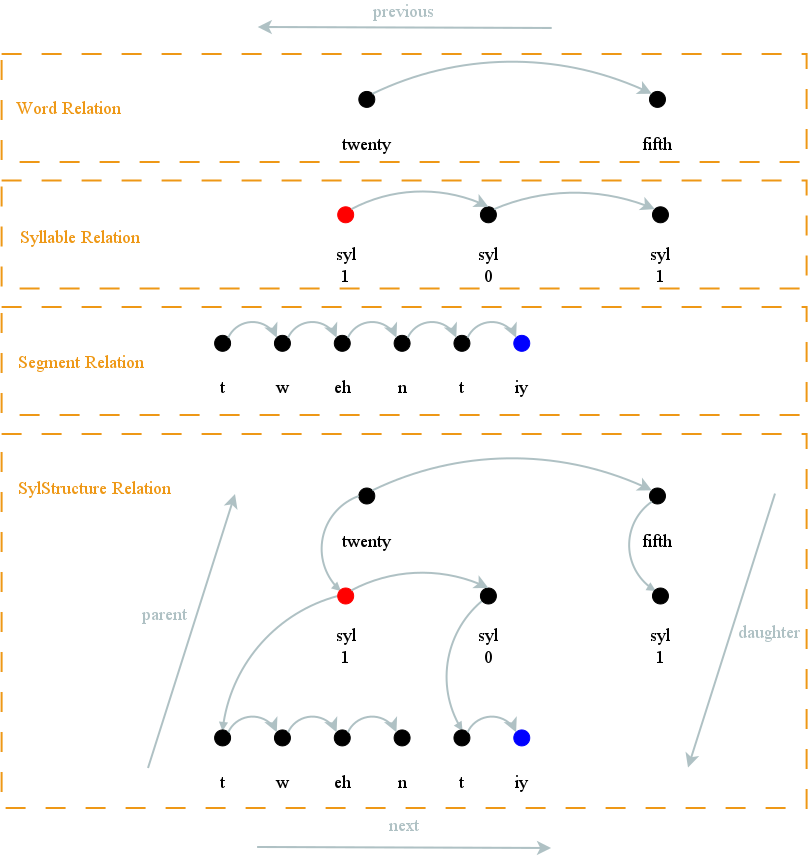
\includegraphics[width=1\columnwidth]{hrg.png}
    \end{column}	
  \end{columns}
\end{frame}
